\documentclass{article}
\usepackage[utf8]{inputenc}
\usepackage{tikz}
\usepackage{amstext}
\usepackage[scale=0.75,top=1cm]{geometry}
\begin{document}
\begin{titlepage}
    \begin{center}
        \vspace*{1cm}

        \Huge
        \textbf{PDL: Práctica Procesador}
        
        \vspace{0.5cm}
        \large
        Procesador JavaScript-PDL
        
        \vspace{3cm}
       
        \textbf{
            Serrano,Arrese Francisco Javier\\
            Cañibano,Lopez Alberto\\
            Vallejo,Collados Jesús
            }
            
        \vspace{8cm}
    
        \large
        Procesadores de Lenguajes\\
        Universidad Politécnica de Madrid\\
        Curso 2020-2021
        
    \end{center}
\end{titlepage}
\newpage
\begin{center}
    PALABRAS RESERVADAS
\end{center}
\fbox{%
  \parbox{\textwidth}{
     alert\\
     boolean\\
     else\\ 
     function\\
     if\\
     input\\
     let\\
     number\\
     return\\
     string\\
     while\\
     false\\
     true\\
     do  
  }
}
\begin{center}
    TOKENS
\end{center}
\fbox{%
  \parbox{\textwidth}{
    \begin{tabular}{l|l}
        alert	            &\textless alert, \textgreater\\
        boolean	            &\textless boolean, \textgreater\\
        else	            &\textless  else, \textgreater\\
        function	        &\textless function, \textgreater\\
        if	                &\textless if, \textgreater\\
        input	            &\textless input, \textgreater\\
        let	                &\textless let, \textgreater\\
        number	            &\textless number, \textgreater\\
        return	            &\textless return, \textgreater\\
        string	            &\textless string, \textgreater\\
        while	            &\textless while, \textgreater\\
        false	            &\textless false, \textgreater\\
        true	            &\textless true, \textgreater\\
        do	                &\textless do, \textgreater\\
        autoInc	            &\textless Autoincremento (++), \textgreater\\
        Número	            &\textless constante entera, \textgreater\\
        Posición(Número)	&\textless Cadena ('), \textgreater\\
        Número	            &\textless Identificador, \textgreater\\
        equal	            &\textless =, \textgreater\\
        colon	            &\textless ,, \textgreater\\
        semicolon	        &\textless ;, \textgreater\\
        openPar	            &\textless (, \textgreater\\
        closePar	        &\textless ), \textgreater\\
        openBraq	        &\textless \{, \textgreater\\
        closeBraq	        &\textless \}, \textgreater\\
        plus	            &\textless +, \textgreater\\
        minus	            &\textless -, \textgreater\\
        and	                &\textless \&\&, \textgreater\\
        not	                &\textless !, \textgreater\\
        notEquals	        &\textless !=, \textgreater\\
        equals	            &\textless ==, \textgreater
        
    \end{tabular}
  }
}
\newpage
\begin{center}
    GRAMÁTICA
\end{center}

\begin{verbatim}
S:--> del S | dA | lB | +C | -D | /F  | ( | ) | { | } | =G | !G | , | ; | &H | 'J
A:--> dA |lambda
B:--> lB | dB | _B | lambda  
C:--> + | lambda
D:--> - | lambda
F:--> *E
E:--> cE | *I | /
I:--> *I | c'E
G:--> = | lambda
H:--> &
J:--> eJ | '


d -- digito
l -- letra minuscula
del -- delimitador(blanco, tab, EOL)
c -- caracteres - (*)
c' -- caracteres - (*/)
e -- caracteres - (')
\end{verbatim}
\newpage
\begin{center}
AUTÓMATA FINITO DETERMINISTA
\end{center}

%\vspace*{1cm}
\fbox{%
  \parbox{\textwidth}{
    \begin{tabular}{l|l}
      d     &Dígito\\
      l     &Letra\\
      del   &Delimitador\\
      c     &Caracteres -\{*\}\\
      c'    &Caracteres -\{*/\}\\
      e     &Caracteres -\{'\}\\
      o.c.  &Otro Caracter
    \end{tabular}
  }
}
\vspace*{1cm}

\begin{center}
    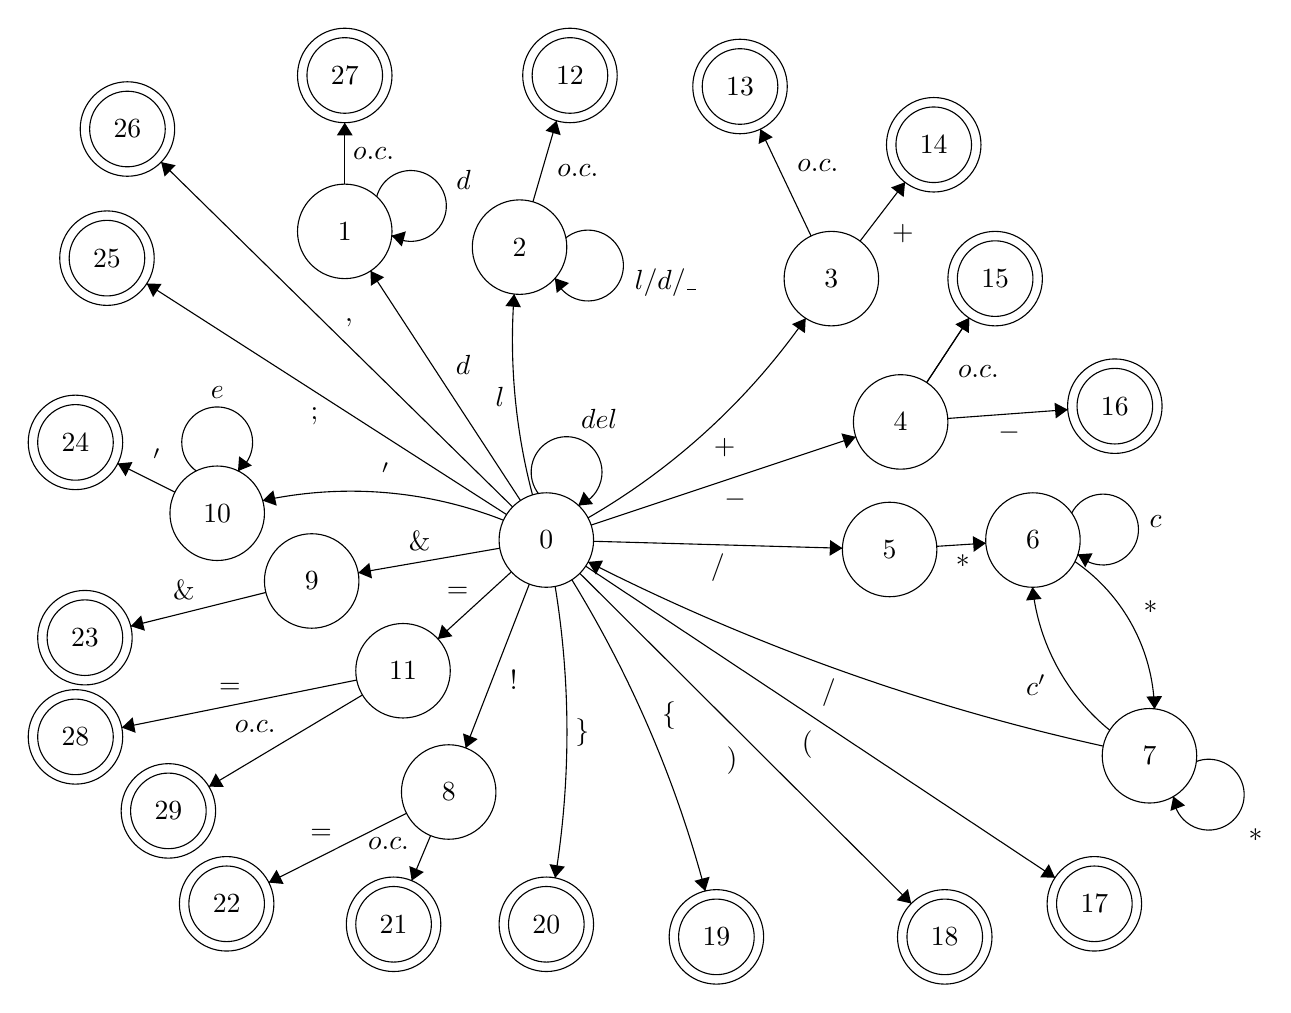
\begin{tikzpicture}[scale=0.2]
    \tikzstyle{every node}+=[inner sep=0pt]
    \draw [black] (34.3,-32) circle (3);
    \draw (34.3,-32) node {$0$};
    \draw [black] (21.5,-12.4) circle (3);
    \draw (21.5,-12.4) node {$1$};
    \draw [black] (21.5,-2.5) circle (3);
    \draw (21.5,-2.5) node {$27$};
    \draw [black] (21.5,-2.5) circle (2.4);
    \draw [black] (32.6,-13.4) circle (3);
    \draw (32.6,-13.4) node {$2$};
    \draw [black] (35.8,-2.5) circle (3);
    \draw (35.8,-2.5) node {$12$};
    \draw [black] (35.8,-2.5) circle (2.4);
    \draw [black] (52.4,-15.4) circle (3);
    \draw (52.4,-15.4) node {$3$};
    \draw [black] (46.6,-3.2) circle (3);
    \draw (46.6,-3.2) node {$13$};
    \draw [black] (46.6,-3.2) circle (2.4);
    \draw [black] (58.9,-6.9) circle (3);
    \draw (58.9,-6.9) node {$14$};
    \draw [black] (58.9,-6.9) circle (2.4);
    \draw [black] (56.8,-24.5) circle (3);
    \draw (56.8,-24.5) node {$4$};
    \draw [black] (62.8,-15.4) circle (3);
    \draw (62.8,-15.4) node {$15$};
    \draw [black] (62.8,-15.4) circle (2.4);
    \draw [black] (70.4,-23.5) circle (3);
    \draw (70.4,-23.5) node {$16$};
    \draw [black] (70.4,-23.5) circle (2.4);
    \draw [black] (56.1,-32.6) circle (3);
    \draw (56.1,-32.6) node {$5$};
    \draw [black] (72.6,-45.7) circle (3);
    \draw (72.6,-45.7) node {$7$};
    \draw [black] (65.2,-32) circle (3);
    \draw (65.2,-32) node {$6$};
    \draw [black] (69.1,-55.1) circle (3);
    \draw (69.1,-55.1) node {$17$};
    \draw [black] (69.1,-55.1) circle (2.4);
    \draw [black] (59.6,-57.2) circle (3);
    \draw (59.6,-57.2) node {$18$};
    \draw [black] (59.6,-57.2) circle (2.4);
    \draw [black] (45.1,-57.2) circle (3);
    \draw (45.1,-57.2) node {$19$};
    \draw [black] (45.1,-57.2) circle (2.4);
    \draw [black] (34.3,-56.4) circle (3);
    \draw (34.3,-56.4) node {$20$};
    \draw [black] (34.3,-56.4) circle (2.4);
    \draw [black] (28.1,-48) circle (3);
    \draw (28.1,-48) node {$8$};
    \draw [black] (24.6,-56.4) circle (3);
    \draw (24.6,-56.4) node {$21$};
    \draw [black] (24.6,-56.4) circle (2.4);
    \draw [black] (14,-55.1) circle (3);
    \draw (14,-55.1) node {$22$};
    \draw [black] (14,-55.1) circle (2.4);
    \draw [black] (19.4,-34.6) circle (3);
    \draw (19.4,-34.6) node {$9$};
    \draw [black] (5,-38.2) circle (3);
    \draw (5,-38.2) node {$23$};
    \draw [black] (5,-38.2) circle (2.4);
    \draw [black] (13.4,-30.3) circle (3);
    \draw (13.4,-30.3) node {$10$};
    \draw [black] (4.4,-25.8) circle (3);
    \draw (4.4,-25.8) node {$24$};
    \draw [black] (4.4,-25.8) circle (2.4);
    \draw [black] (6.4,-14.1) circle (3);
    \draw (6.4,-14.1) node {$25$};
    \draw [black] (6.4,-14.1) circle (2.4);
    \draw [black] (7.7,-5.9) circle (3);
    \draw (7.7,-5.9) node {$26$};
    \draw [black] (7.7,-5.9) circle (2.4);
    \draw [black] (25.2,-40.3) circle (3);
    \draw (25.2,-40.3) node {$11$};
    \draw [black] (4.4,-44.5) circle (3);
    \draw (4.4,-44.5) node {$28$};
    \draw [black] (4.4,-44.5) circle (2.4);
    \draw [black] (10.3,-49.2) circle (3);
    \draw (10.3,-49.2) node {$29$};
    \draw [black] (10.3,-49.2) circle (2.4);
    \draw [black] (33.799,-29.054) arc (217.38765:-70.61235:2.25);
    \draw (37.66,-24.95) node [above] {$del$};
    \fill [black] (36.33,-29.81) -- (37.27,-29.72) -- (36.67,-28.93);
    \draw [black] (32.66,-29.49) -- (23.14,-14.91);
    \fill [black] (23.14,-14.91) -- (23.16,-15.86) -- (24,-15.31);
    \draw (28.52,-20.88) node [right] {$d$};
    \draw [black] (23.526,-10.204) arc (165.03751:-122.96249:2.25);
    \draw (28.55,-9.13) node [right] {$d$};
    \fill [black] (24.48,-12.67) -- (25.12,-13.36) -- (25.38,-12.4);
    \draw [black] (21.5,-9.4) -- (21.5,-5.5);
    \fill [black] (21.5,-5.5) -- (21,-6.3) -- (22,-6.3);
    \draw (22,-7.45) node [right] {$o.c.$};
    \draw [black] (33.422,-29.132) arc (-165.21371:-184.34188:38.536);
    \fill [black] (32.26,-16.38) -- (31.7,-17.14) -- (32.69,-17.22);
    \draw (31.68,-22.88) node [left] {$l$};
    \draw [black] (35.531,-12.82) arc (128.93151:-159.06849:2.25);
    \draw (39.88,-15.67) node [right] {$l/d/\_$};
    \fill [black] (34.84,-15.37) -- (34.96,-16.31) -- (35.74,-15.68);
    \draw [black] (33.45,-10.52) -- (34.95,-5.38);
    \fill [black] (34.95,-5.38) -- (34.25,-6.01) -- (35.21,-6.29);
    \draw (34.97,-8.54) node [right] {$o.c.$};
    \draw [black] (50.768,-17.917) arc (-34.95047:-59.99997:43.235);
    \fill [black] (50.77,-17.92) -- (49.9,-18.29) -- (50.72,-18.86);
    \draw (45.63,-25.5) node [below] {$+$};
    \draw [black] (51.11,-12.69) -- (47.89,-5.91);
    \fill [black] (47.89,-5.91) -- (47.78,-6.85) -- (48.68,-6.42);
    \draw (50.21,-8.24) node [right] {$o.c.$};
    \draw [black] (54.22,-13.02) -- (57.08,-9.28);
    \fill [black] (57.08,-9.28) -- (56.19,-9.61) -- (56.99,-10.22);
    \draw (56.22,-12.56) node [right] {$+$};
    \draw [black] (37.15,-31.05) -- (53.95,-25.45);
    \fill [black] (53.95,-25.45) -- (53.04,-25.23) -- (53.35,-26.18);
    \draw (46.29,-28.78) node [below] {$-$};
    \draw [black] (58.45,-22) -- (61.15,-17.9);
    \fill [black] (61.15,-17.9) -- (60.29,-18.3) -- (61.13,-18.85);
    \draw (60.41,-21.28) node [right] {$o.c.$};
    \draw [black] (59.79,-24.28) -- (67.41,-23.72);
    \fill [black] (67.41,-23.72) -- (66.57,-23.28) -- (66.65,-24.28);
    \draw (63.69,-24.55) node [below] {$-$};
    \draw [black] (58.45,-22) -- (61.15,-17.9);
    \fill [black] (61.15,-17.9) -- (60.29,-18.3) -- (61.13,-18.85);
    \draw [black] (37.3,-32.08) -- (53.1,-32.52);
    \fill [black] (53.1,-32.52) -- (52.32,-32) -- (52.29,-33);
    \draw (45.19,-32.82) node [below] {$/$};
    \draw [black] (59.09,-32.4) -- (62.21,-32.2);
    \fill [black] (62.21,-32.2) -- (61.38,-31.75) -- (61.44,-32.75);
    \draw (60.74,-32.86) node [below] {$*$};
    \draw [black] (67.655,-30.296) arc (152.4872:-135.5128:2.25);
    \draw (72.57,-30.82) node [right] {$c$};
    \fill [black] (68.05,-32.91) -- (68.52,-33.73) -- (68.99,-32.84);
    \draw [black] (67.862,-33.365) arc (55.48576:1.26528:11.672);
    \fill [black] (72.92,-42.73) -- (73.4,-41.91) -- (72.4,-41.94);
    \draw (72.19,-36.26) node [right] {$*$};
    \draw [black] (70.082,-44.08) arc (-129.12273:-174.12623:13.492);
    \fill [black] (65.17,-34.99) -- (64.76,-35.84) -- (65.75,-35.74);
    \draw (66.05,-41.2) node [left] {$c'$};
    \draw [black] (75.566,-46.065) arc (110.70899:-177.29101:2.25);
    \draw (78.86,-50.73) node [right] {$*$};
    \fill [black] (74.11,-48.28) -- (73.93,-49.2) -- (74.86,-48.85);
    \draw [black] (69.664,-45.085) arc (-102.44672:-116.91778:137.886);
    \fill [black] (36.96,-33.39) -- (37.45,-34.2) -- (37.9,-33.3);
    \draw (52.23,-40.79) node [below] {$/$};
    \draw [black] (36.8,-33.66) -- (66.6,-53.44);
    \fill [black] (66.6,-53.44) -- (66.21,-52.58) -- (65.66,-53.42);
    \draw (50.87,-44.05) node [below] {$($};
    \draw [black] (36.43,-34.12) -- (57.47,-55.08);
    \fill [black] (57.47,-55.08) -- (57.26,-54.16) -- (56.55,-54.87);
    \draw (46.09,-45.08) node [below] {$)$};
    \draw [black] (35.921,-34.524) arc (31.54446:14.85272:74.061);
    \fill [black] (44.39,-54.29) -- (44.67,-53.38) -- (43.7,-53.64);
    \draw (41.61,-43.14) node [right] {$\{$};
    \draw [black] (34.86,-34.947) arc (9.27057:-9.27057:57.438);
    \fill [black] (34.86,-53.45) -- (35.48,-52.74) -- (34.5,-52.58);
    \draw (36.11,-44.2) node [right] {$\}$};
    \draw [black] (33.22,-34.8) -- (29.18,-45.2);
    \fill [black] (29.18,-45.2) -- (29.94,-44.64) -- (29.01,-44.28);
    \draw (31.95,-40.85) node [right] {$!$};
    \draw [black] (26.95,-50.77) -- (25.75,-53.63);
    \fill [black] (25.75,-53.63) -- (26.52,-53.08) -- (25.6,-52.7);
    \draw (25.61,-51.27) node [left] {$o.c.$};
    \draw [black] (25.42,-49.35) -- (16.68,-53.75);
    \fill [black] (16.68,-53.75) -- (17.62,-53.84) -- (17.17,-52.94);
    \draw (20,-51.05) node [above] {$=$};
    \draw [black] (31.34,-32.52) -- (22.36,-34.08);
    \fill [black] (22.36,-34.08) -- (23.23,-34.44) -- (23.06,-33.45);
    \draw (26.25,-32.68) node [above] {$\&$};
    \draw [black] (16.49,-35.33) -- (7.91,-37.47);
    \fill [black] (7.91,-37.47) -- (8.81,-37.76) -- (8.57,-36.79);
    \draw (11.28,-35.81) node [above] {$\&$};
    \draw [black] (16.289,-29.498) arc (102.25681:68.44282:26.374);
    \fill [black] (16.29,-29.5) -- (17.18,-29.82) -- (16.96,-28.84);
    \draw (24.11,-28.44) node [above] {$'$};
    \draw [black] (12.077,-27.62) arc (234:-54:2.25);
    \draw (13.4,-23.05) node [above] {$e$};
    \fill [black] (14.72,-27.62) -- (15.6,-27.27) -- (14.79,-26.68);
    \draw [black] (10.72,-28.96) -- (7.08,-27.14);
    \fill [black] (7.08,-27.14) -- (7.58,-27.95) -- (8.02,-27.05);
    \draw (9.57,-27.55) node [above] {$'$};
    \draw [black] (31.77,-30.38) -- (8.93,-15.72);
    \fill [black] (8.93,-15.72) -- (9.33,-16.57) -- (9.87,-15.73);
    \draw (19.57,-23.55) node [below] {$;$};
    \draw [black] (32.16,-29.9) -- (9.84,-8);
    \fill [black] (9.84,-8) -- (10.06,-8.92) -- (10.76,-8.2);
    \draw (21.77,-18.47) node [above] {$,$};
    \draw [black] (22.26,-40.89) -- (7.34,-43.91);
    \fill [black] (7.34,-43.91) -- (8.22,-44.24) -- (8.03,-43.26);
    \draw (14.2,-41.81) node [above] {$=$};
    \draw [black] (22.62,-41.84) -- (12.88,-47.66);
    \fill [black] (12.88,-47.66) -- (13.82,-47.68) -- (13.31,-46.82);
    \draw (15.81,-44.25) node [above] {$o.c.$};
    \draw [black] (32.08,-34.02) -- (27.42,-38.28);
    \fill [black] (27.42,-38.28) -- (28.34,-38.11) -- (27.67,-37.37);
    \draw (28.67,-35.66) node [above] {$=$};
    \end{tikzpicture}
    \end{center}
\vspace{2cm}
\newpage
\begin{center}
ACCIONES SEMÁNTICAS\\
\end{center}
\noindent
\textbf{Leer:}Se lee en todos los estados menos en los que pone o.c.\\
\textbf{Errores}:  Cualquier transicion no declarada dara error.\\

\textbf{Caso 0-1:}
\begin{verbatim}
    if siguienteCaracter==d
        numero=valor(d)
    else
        Error("SIMBOLO NO RECONOCIDO")
\end{verbatim}

\textbf{Caso 1-1:}
\begin{verbatim}
    if siguienteCaracter==d
        numero=numero+d
    else 
        Error("SIMBOLO NO RECONOCIDO")
\end{verbatim}

\textbf{Caso 1-27:}
\begin{verbatim}
    GenerarToken(wholeConst,numero)
\end{verbatim}

\textbf{Caso 0-2:}
\begin{verbatim}
    if siguienteCaracter==l 
        lexema=l
    else 
        Error("SIMBOLO NO RECONOCIDO")
\end{verbatim}

\textbf{Caso 2-2:}
\begin{verbatim}
    if siguienteCaracter== l | d | '_' 
        lexema=lexema+(l|d|'_')
    else 
        Error("SIMBOLO NO RECONOCIDO")
\end{verbatim}

\textbf{Caso 2-12:}
\begin{verbatim}
    GenerarToken(ID,posicionTablaSimbolos)
\end{verbatim}

\textbf{Caso 0-3:}
\begin{verbatim}
    if siguienteCaracter=='+'
        //Nada
    else
        Error("SIMBOLO NO RECONOCIDO")
\end{verbatim}

\textbf{Caso 3-13:}
\begin{verbatim}
    GenerarToken(aritOp,plus)
\end{verbatim}

\textbf{Caso 3-14:}
\begin{verbatim}
    if siguienteCaracter=='+'
        GenerarToken(autoIncOp,autoinc)
    else 
        Error("SIMBOLO NO RECONOCIDO")
\end{verbatim}

\textbf{Caso 0-4:}
\begin{verbatim}
    if siguienteCaracter=='-'
        //Nada
    else
        Error("SIMBOLO NO RECONOCIDO")
\end{verbatim}

\textbf{Caso 4-15:}
\begin{verbatim}
    GenerarToken(aritOp,minus)
\end{verbatim}

\textbf{Caso 4-16:}
\begin{verbatim}
    if siguienteCarcter=='-'
        GenerarToken(autoIncOp,autoinc)
    else 
        Error("SIMBOLO NO RECONOCIDO")
\end{verbatim}

\textbf{Caso 0-5:}
\begin{verbatim}
    if siguienteCaracter=='/'
        //NADA
    else
        Error("SIMBOLO NO RECONOCIDO")
\end{verbatim}

\textbf{Caso 5-6:}
\begin{verbatim}
    if siguienteCaracater=='*'
        //NADA
    else
        Error("SIMBOLO NO RECONOCIDO")
\end{verbatim}

\textbf{Caso 6-6:}
\begin{verbatim}
    if siguienteCaracater=='c'
        //NADA
    else
        Error("SIMBOLO NO RECONOCIDO")
\end{verbatim}

\textbf{Caso 6-7:}
\begin{verbatim}
    if siguienteCaracater=='*'
         //NADA
    else
         Error("SIMBOLO NO RECONOCIDO")
\end{verbatim}
\newpage
\textbf{Caso 7-6:}
\begin{verbatim}
    if siguienteCaracater=='c''
        //NADA
    else
        Error("SIMBOLO NO RECONOCIDO")
\end{verbatim}

\textbf{Caso 7-0:}
\begin{verbatim}
    if siguienteCaracater=='/'
        //NADA
    else
        Error("SIMBOLO NO RECONOCIDO")
\end{verbatim}

\textbf{Caso 0-26:}
\begin{verbatim}
    if siguienteCaracter==','
        GenerarToken(separator,colon)
    else
        Error("SIMBOLO NO RECONOCIDO")
\end{verbatim}

\textbf{Caso 0-25:}
\begin{verbatim}
    if siguienteCaracter==';'
        GenerarToken(separator,semicolon)
    else
        Error("SIMBOLO NO RECONOCIDO") )
\end{verbatim}

\textbf{Caso 0-20:}
\begin{verbatim}
    if siguienteCaracter=='}'
        GenerarToken(separator,closeBraq)
    else
        Error("SIMBOLO NO RECONOCIDO")  
\end{verbatim}

\textbf{Caso 0-19:}
\begin{verbatim}
    if siguienteCaracter=='{'
        GenerarToken(separator,openBraq)
    else
        Error("SIMBOLO NO RECONOCIDO")
\end{verbatim}

\textbf{Caso 0-18:}
\begin{verbatim}
    if siguienteCaracter==')'
        GenerarToken(separator,closePar)
    else
        Error("SIMBOLO NO RECONOCIDO")  
\end{verbatim}

\textbf{Caso 0-17:}
\begin{verbatim}
    if siguienteCaracter=='('
        GenerarToken(separator,openPar)
    else
        Error("SIMBOLO NO RECONOCIDO")
\end{verbatim}
\newpage
\textbf{Caso 0-10:}
\begin{verbatim}
    if siguienteCaracter=='''
        lexema=''
    else
        Error ("SIMBOLO NO RECONOCIDO)
\end{verbatim}

\textbf{Caso 10-10:}
\begin{verbatim}
    if siguienteCaracter==e
        lexema=lexema+e
    else 
        Error ("SIMBOLO NO RECONOCIDO)
\end{verbatim}

\textbf{Caso 10-24:}
\begin{verbatim}
    if siguienteCaracater=='''
        GenerarToken(chain,posicionTablaSimbolos)//revisar
    else 
        Error ("SIMBOLO NO RECONOCIDO")
\end{verbatim}

\textbf{Caso 0-8:}
\begin{verbatim}
    if siguienteCaracter=='!'
    
    else 
        Error ("SIMBOLO NO RECONOCIDO")
\end{verbatim}

\textbf{Caso 8-21:}
\begin{verbatim}
        GenerarToken(logOp,not)
\end{verbatim}

\textbf{Caso 8-22:}
\begin{verbatim}
    if siguienteCaracater == '='
        GenerarToken(relOp,notEquals)
    else 
        Error ("SIMBOLO NO RECONOCIDO")  
\end{verbatim}

\textbf{Caso 0-11:}
\begin{verbatim}
    if siguienteCaracater == '='

    else 
        Error ("SIMBOLO NO RECONOCIDO")  
\end{verbatim}

\textbf{Caso 11-28:}
\begin{verbatim}
    if siguienteCaracater == '='
        GenerarToken(relOp,equals)
    else 
        Error ("SIMBOLO NO RECONOCIDO")  
\end{verbatim}

\textbf{Caso 11-29:}
\begin{verbatim}
        GenerarToken(asigOp,equal)
\end{verbatim}
\newpage
\textbf{Caso 0-9:}
\begin{verbatim}
    if siguienteCaracter == '&'
        
    else
        Error("SIMBOLO NO RECONOCIDO")
\end{verbatim}

\textbf{Caso 9-23:}
\begin{verbatim}
    if siguienteCaracter == '&'
        GenerarToken(logOp,and)
    else
        Error("SIMBOLO NO RECONOCIDO")
\end{verbatim}

\vspace*{1cm}

\begin{center}
    TABLA DE SIMBOLOS\\
    \end{center}
\vspace*{1cm}
El valor de los atributos y numero de tabla seran corregidos con el valor real mas adelante.
\begin{verbatim}
    Contenido Tabla Símbolos # N :
    * LEXEMA : 'x'
      ATRIBUTOS :
        + tipo: unknown
        + despl: unknown
    
\end{verbatim}


\end{document}